\subsection{CA}
\subsubsection{Validazione requisiti obbligatori e desiderabili}
Unico consuntivo della macrofase Customer Acceptance.
\paragraph{Consuntivo Orario}
\begin{center}
	\renewcommand{\arraystretch}{1.8} %aumento ampiezza righe
	\begin{tabular}{ |m{8em}|c|c|c|c|c|c|c| }
	\hline
	\textbf{Membro} & \textbf{Re} & \textbf{Am} &  \textbf{An} &  \textbf{Pt} &  \textbf{Pg} &  \textbf{Ve} &  \textbf{Totale}\\
    \hline
    Irene Benetazzo   & - (-2) & 3 & - & - (-1) & - & 11 (+3) & \textbf{14} \\
    \hline
    Tommaso Berlaffa  & - & 3 (+1) & - & - (-2) & 2 & 10 (+1) & \textbf{15} \\
    \hline
    Mattia Episcopo   & 1 & 2 (+2) & - & - & - (-2) & 9 & \textbf{12}  \\
    \hline
    Pietro Macrì      & - & 3 (+1) & - & - (-1) & 3 & 11 & \textbf{17} \\
    \hline
    Qi Fan Andrea Pan & 1 (+1) & - (-1) & - & - (-3) & - (-1) & 15 (+4) & \textbf{16} \\
    \hline
    Matteo Pillon     & - & 3 (+3) & - & - (-2) & - (-1) & 11 & \textbf{14} \\
    \hline
    Samuele Rizzato   & 3 (+1) & 1 (-1) & - & - (-1) & - (-1) & 8 (+2) & \textbf{12} \\
    \hline
    \textbf{Totale ore} & \textbf{5} & \textbf{15} (+5) & \textbf{0} &  \textbf{0} (-10) &  \textbf{5} (-5) &  \textbf{75} (+10) &  \textbf{100}\\
    \hline
	\end{tabular}
\end{center}

\begin{figure}[H]
    \centering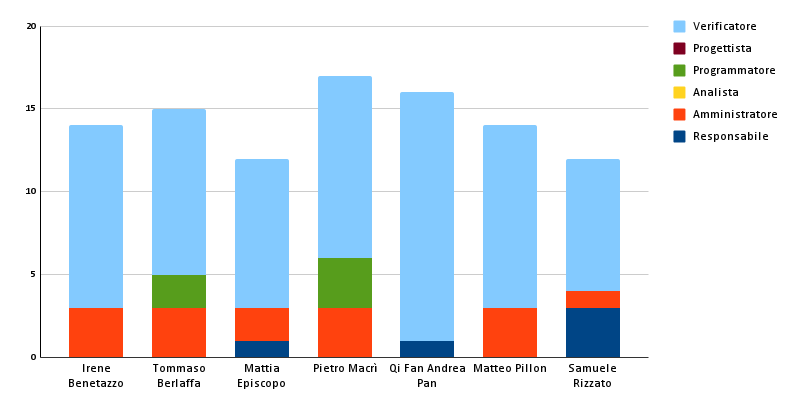
\includegraphics[width=\textwidth, height=\textheight,keepaspectratio]{images/consuntivo/CA-validazione-dei-requisiti-obbligatori-e-desiderabili-orario.png}
    \caption{CA - Customer Acceptance - Validazione dei requisiti obbligatori e desiderabili - consuntivo ripartizione oraria}
\end{figure}

\paragraph{Consuntivo Economico}
\begin{center}
	\renewcommand{\arraystretch}{1.8}
	\begin{tabular}{ |m{6em}|c|c|c|c|c|c|c| }
	\hline
	\textbf{Ruolo} & \textbf{Re} & \textbf{Am} &  \textbf{An} &  \textbf{Pt} &  \textbf{Pg} &  \textbf{Ve} &  \textbf{Totale}\\
    \hline
    Totale ore & 5 & 15 & 0 & 0 & 5 & 75 & \textbf{100}\\
    \hline
    Costo \euro/h & 30\euro/h & 20\euro/h & 25\euro/h & 25\euro/h & 15\euro/h & 15\euro/h & \\
    \hline
    \textbf{Totale costo} & \textbf{150\euro} & \textbf{300\euro} &  \textbf{0\euro} & \textbf{0\euro} &  \textbf{75\euro} &  \textbf{1125\euro} &  \textbf{1650\euro} \\
    &  & (+100\euro) &  & (-250\euro) & (-75\euro) & (+150\euro) & (-75\euro) \\
    \hline
	\end{tabular}

    \begin{figure}[H]
        \centering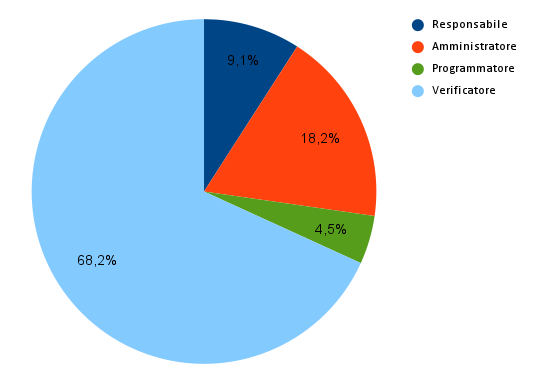
\includegraphics[width=0.7\textwidth, height=0.7\textheight, keepaspectratio]{images/consuntivo/CA-validazione-dei-requisiti-obbligatori-e-desiderabili-costo.png}
        \caption{CA - Customer Acceptance - Validazione dei requisiti obbligatori e desiderabili - consuntivo ripartizione economica}
    \end{figure}
\end{center}

\paragraph{Considerazioni} \hfill \break
\begin{center}
	\renewcommand{\arraystretch}{1.8}
	\begin{tabular}{ | l |c|c| }
    \hline
    & \textbf{Ore} & \textbf{Costo} \\
	\hline
    \textbf{Consuntivo} & 100 & 1650\euro \\
    \hline
    \textbf{Preventivo} & 100 & 1725\euro \\
    \hline
    \textbf{Bilancio macrofase} & - & -75\euro \\
    \hline
    \end{tabular}
\end{center}
Per questo incremento c'è stato un numero alto di ore di verificatore poiché si sono accorpati i due incrementi della fase CA in un unico incremento per rispettare il calendario e terminare
entro il 25-09-2022. Il gruppo nonostante ciò è riuscito a completare le attività pianificate per la fase di validazione anche perché il proponente, durante la riunione
esterna di questa fase, non ha individuato discrepanze con le proprie aspettative. Sono state impiegate più ore di amministratore in quanto non era stata prevista la correzione di alcune parti dei documenti del progetto.
Le ore da progettista e programmatore sono state sovrastimate siccome si pensava di implementare la funzionalità di creazione di una riunione esterna, ma per rispettare il calendario non è stata realizzata. In conclusione
l'incremento è costato meno di quanto preventivato e la fase CA è terminata il 25-09-2022 rispettando il preventivo.